We conduct extensive experiments on five real-world tabular datasets
to evaluate the classification performance (accuracy and AUC) of our
method \textbf{CCRAL}, comparing it with two strong baselines.

\subsection{Datasets}

To create an environment for comprehending counterfactual reasoning
involved in our method \textbf{CCRAL}, we choose five real-world tabular
datasets that have at least one binary feature that intrigues one's
causal thinking. These datasets were often used to evaluate fairness-aware
and causal inference machine learning algorithms \cite{friedler2019comparative,zafar2017parity,nguyen2021fairness}.

Table~\ref{tab:Characteristics-of-datasets} shows characteristics
of each dataset along with the selected treatment feature and the
respective outcome.

\begin{table}
\caption{\label{tab:Characteristics-of-datasets}Characteristics of five tabular
datasets. We denote $N$: the number of samples, $M$: the number
of features, $T$: the treatment feature, and $y$: the class feature.}

\centering{}%
\begin{tabular}{|l|r|r|c|c|c|c|c|c|}
\hline 
\textbf{Dataset} & \textbf{$N$} & \textbf{$M$} & $T$ & \textbf{$T=1$} & \textbf{$T=0$} & \textbf{$y$} & \textbf{$y=1$} & \textbf{$y=0$}\tabularnewline
\hline 
\hline 
\textit{german} & 1,000 & 20 & Sex & ``male'' & ``female'' & Credit & ``good'' & ``bad''\tabularnewline
\hline 
\textit{bank} & 4,521 & 14 & Marriage & ``married'' & ``single'' & Subscription & ``yes'' & ``no''\tabularnewline
\hline 
\textit{twins} & 4,821 & 52 & Weight & ``heavier'' & ``lighter'' & Mortality & ``alive'' & ``death''\tabularnewline
\hline 
\textit{compas} & 4,010 & 10 & Sex & ``male'' & ``female'' & Rearrested & ``no'' & ``yes''\tabularnewline
\hline 
\textit{adult} & 30,162 & 13 & Sex & ``male'' & ``female'' & Income & ``\textgreater 50K'' & ``\textless 50K''\tabularnewline
\hline 
\end{tabular}
\end{table}
\textit{german}: this dataset describes each individual's credit score
whether she/he has a good or bad credit score \cite{dua_graff_19_uci}.
It has 1,000 samples and 20 features. We use \textit{Sex} as the treatment
feature.

\textit{bank}: this dataset is about direct marketing campaigns of
individuals for term deposit subscriptions. The outcome of this data
is whether a person is subscribed or not depending upon the marketing
and duration campaigned. \textit{Marriage} is the treatment feature
in this dataset.

\textit{twins}: this dataset consists of around 5,000 records of twin's
birth collected during the period of 1989-1991 in the U.S. \cite{almond2005costs}.
It is a popular benchmark dataset in causality researches \cite{louizos2017causal}.
The outcome corresponds to the mortality of each twin's during the
first year of birth. We choose twins of the same gender to replicate
the counterfactual. The treatment feature is the twin's\textit{ weight}.

\textit{compas}: this dataset includes a collection of data in Broward
country, Florida about the use of the COMPAS risk assessment tool
and has the data regarding felonies and charges on the degree of the
arrest \cite{angwin2016machine}. This dataset has the treatment feature
\textit{Sex} with an outcome of getting rearrested within two years.

\textit{adult}: this dataset is the collection of individual data
of their income recorded during the 1994 U.S census \cite{kamiran2012decision}.
The outcome is a person's income. If the income is greater than \$50K,
then it is labeled as ``1''. Otherwise it is ``0''. This dataset
has 30,162 samples and 13 features. We select \textit{Sex} as the
treatment feature.

\subsection{Baselines and evaluation}

We compare our method \textbf{CCARL} with two strong baselines.
\begin{enumerate}
\item \textbf{Standard}: this method uses available training samples to
train a classifier.
\item \textbf{Counterfactual}: this method uses the counterfactual samples
of all original training samples in the training process. In other
words, it fixes $\alpha=0.5$ in Equation (\ref{eq:uncertain_region}).
\end{enumerate}
For a fair comparison, we measure the accuracy and AUC of each method
on the same hold-out test set. We also use the same classifier for
all methods, namely the Support Vector Machine (SVM) with the linear
kernel and $C=1$ for the regularization. Note that other machine
learning classifiers can be used with our method. We use the default
search range $[0,0.5]$ for $\alpha$, and set the number of iterations
$K=10$. We evaluate methods on each dataset in five times with different
train-test data splits, and report the averaged accuracy and AUC.

\subsection{Results}

Figure \ref{fig:Classification-accuracy} shows the accuracy of each
method on five datasets. It can be seen that our method \textbf{CCRAL}
is much better than the standard classifier on all datasets. On \textit{german}
(a small dataset), Standard achieves only 61.0\% whereas \textbf{CCRAL}
achieves 70.0\%, resulting in 9\% better. On \textit{adult} (a very
large dataset), the accuracy of Standard is 79.28\% compared to 82.82\%
of our \textbf{CCRAL}. On this dataset, our method achieves around
3\% gains over the standard classifier.

\begin{figure}
\centering{}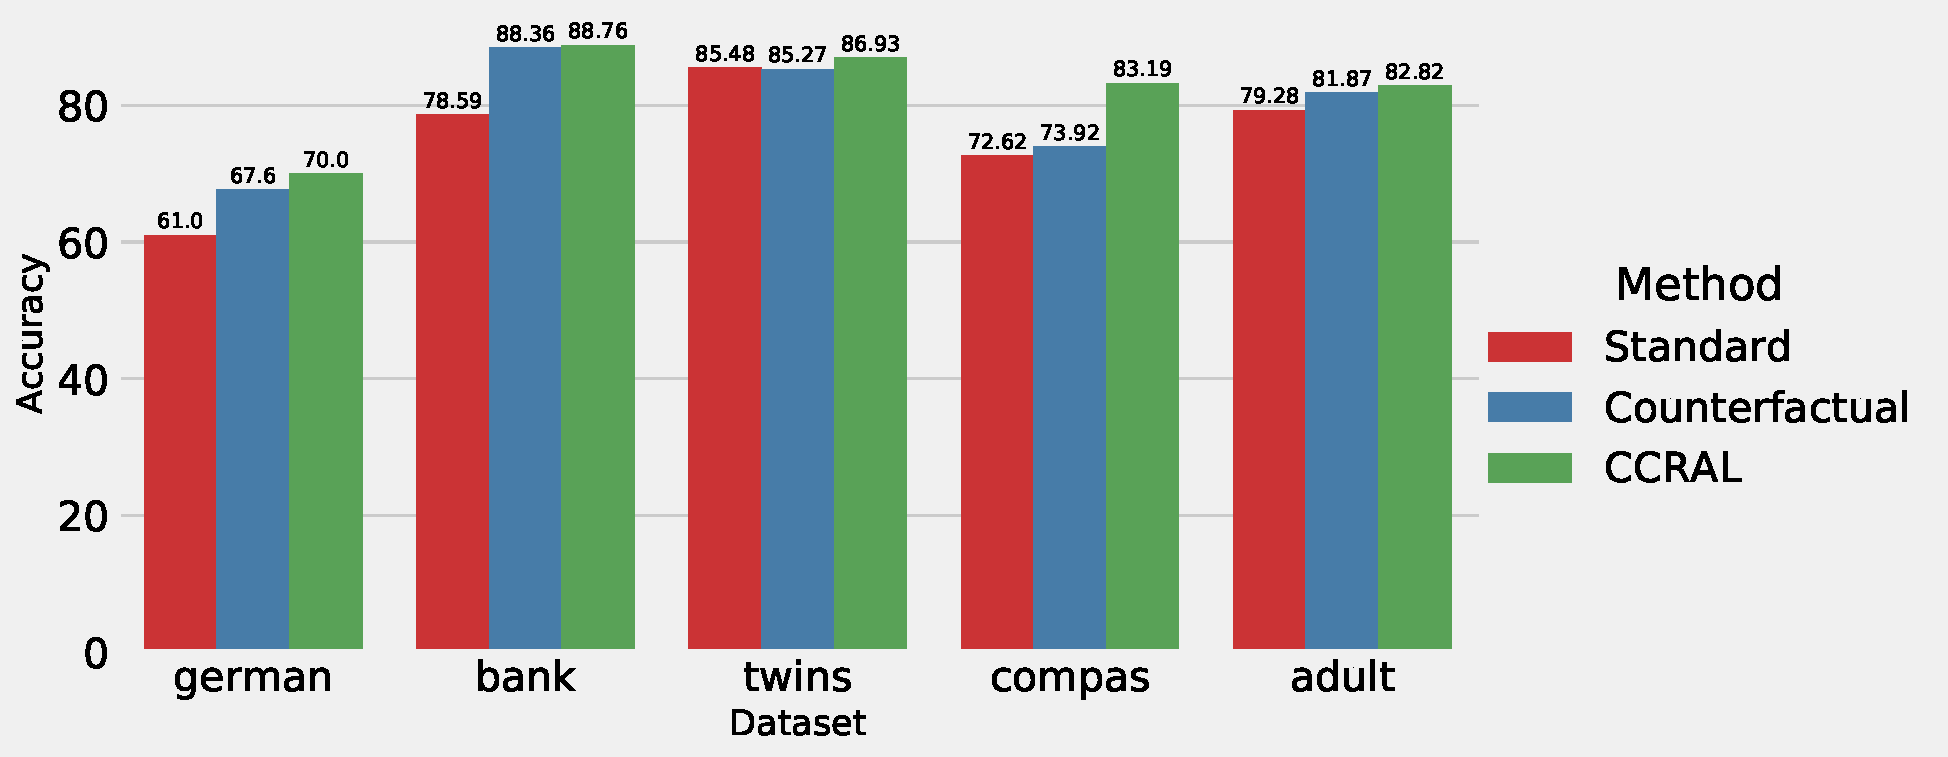
\includegraphics[scale=0.35]{figs/_plot_svm_accuracy}\caption{\label{fig:Classification-accuracy}The averaged classification accuracy
of two baselines Standard, Counterfactual, and our method \textbf{CCRAL}
on each dataset.}
\end{figure}
Compared to the Counterfactual method, \textbf{CCRAL} is comparable
on three datasets \textit{bank}, \textit{twins}, and \textit{adult}
while it is much better on two datasets \textit{german} and \textit{compas}.
This shows that using all counterfactual samples in the training process
was not a good solution since they might add noise to the training
data, as we discussed in Section \ref{subsec:Training-classifier-with}.
Our method which uses active learning to select useful counterfactual
samples is a more efficient approach to train the classifier.

We also report the AUC of each method in Figure \ref{fig:Classification-AUC}.
Our \textbf{CCRAL} is the best method, where it significantly outperforms
two baselines Standard and Counterfactual. \textbf{CCRAL} always outperforms
the standard classifier by a large margin across all datasets. Compared
to Counterfactual, our method shows a great improvement, where it
achieves 3-9\% gains over Counterfactual. Again, this suggests that
using active learning to select useful counterfactual samples is a
much better strategy than using all counterfactual samples for training
the classifier.

\begin{figure}
\begin{centering}
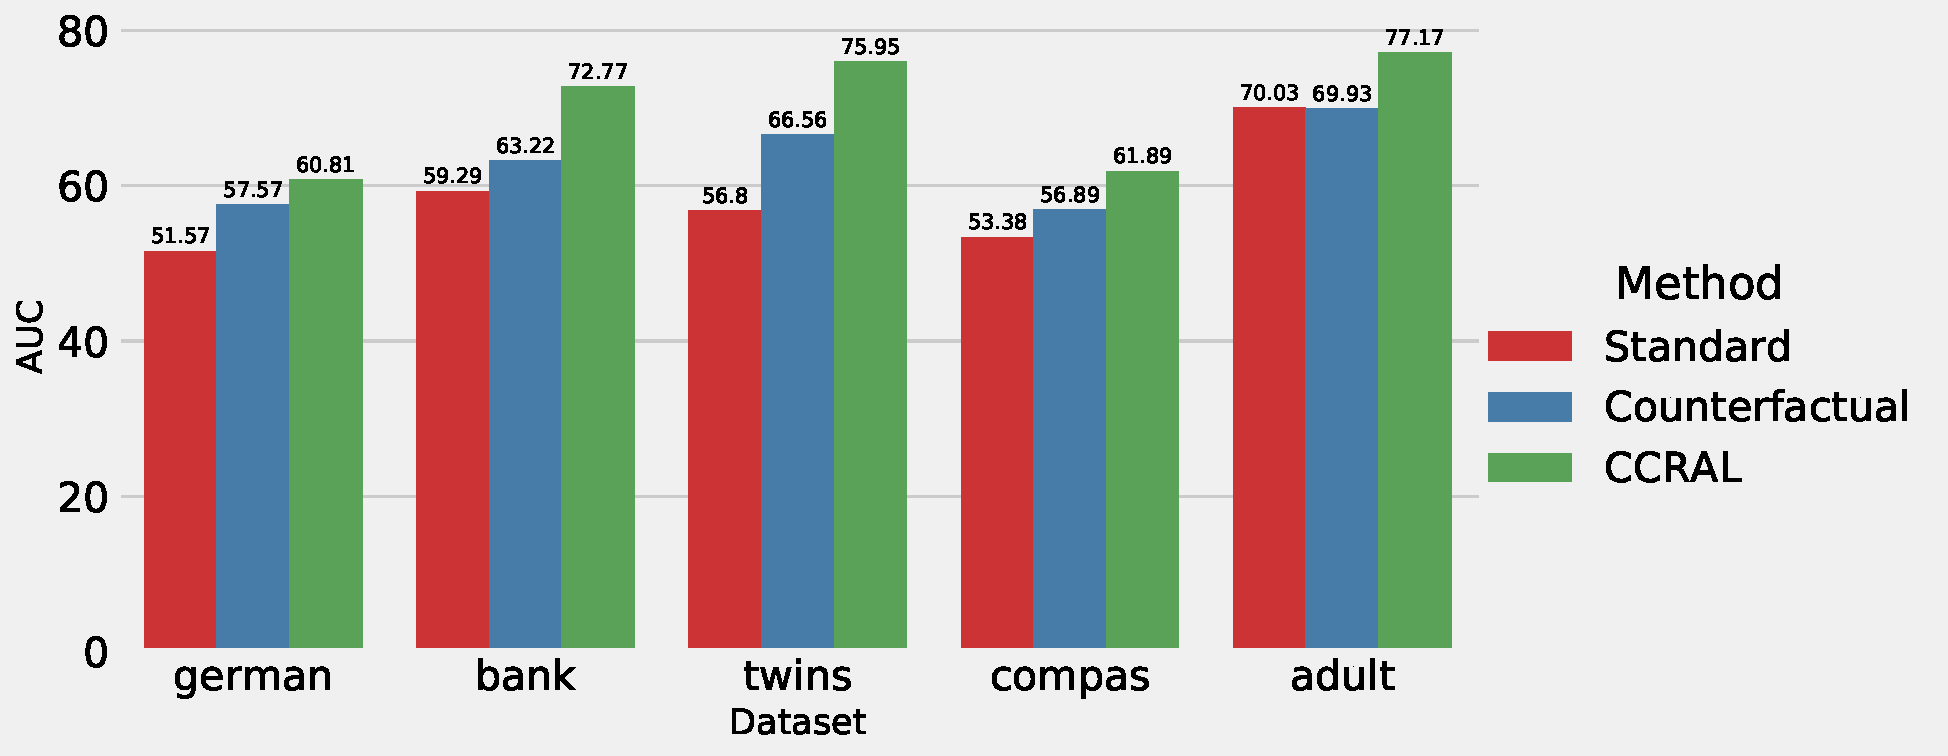
\includegraphics[scale=0.35]{figs/_plot_svm_auc}
\par\end{centering}
\caption{\label{fig:Classification-AUC}The averaged AUC of two baselines Standard,
Counterfactual, and our method \textbf{CCRAL} on each dataset.}
\end{figure}

